\begin{frame}{Methods}
    \begin{itemize}
        \item \textbf{Distortion–free decoding (Exp-Min).}
              For a language-model next–token distribution
              \(p:\mathcal V\!\to\![0,1]\) and a private key
              \(\xi_i\!\sim\!\text{Uniform}(0,1)^{|\mathcal V|}\),
              select
              \[
                  t_i^\star \;=\;
                  \operatorname*{arg\,min}_{t\in\mathcal V}
                  \Bigl\{-\frac{\ln\xi_{i,t}}{p(t)}\Bigr\},
              \]
              which samples \(\textstyle t_i^\star\sim p\) \emph{without
                  altering \(p\)}.
        \item \textbf{Inverse-transform sampling} (ITS) baseline
        \item Robustness with \textbf{Levenshtein distance}

    \end{itemize}
\end{frame}

\begin{frame}{Method comparisons}
    \begin{figure}
        \centering
        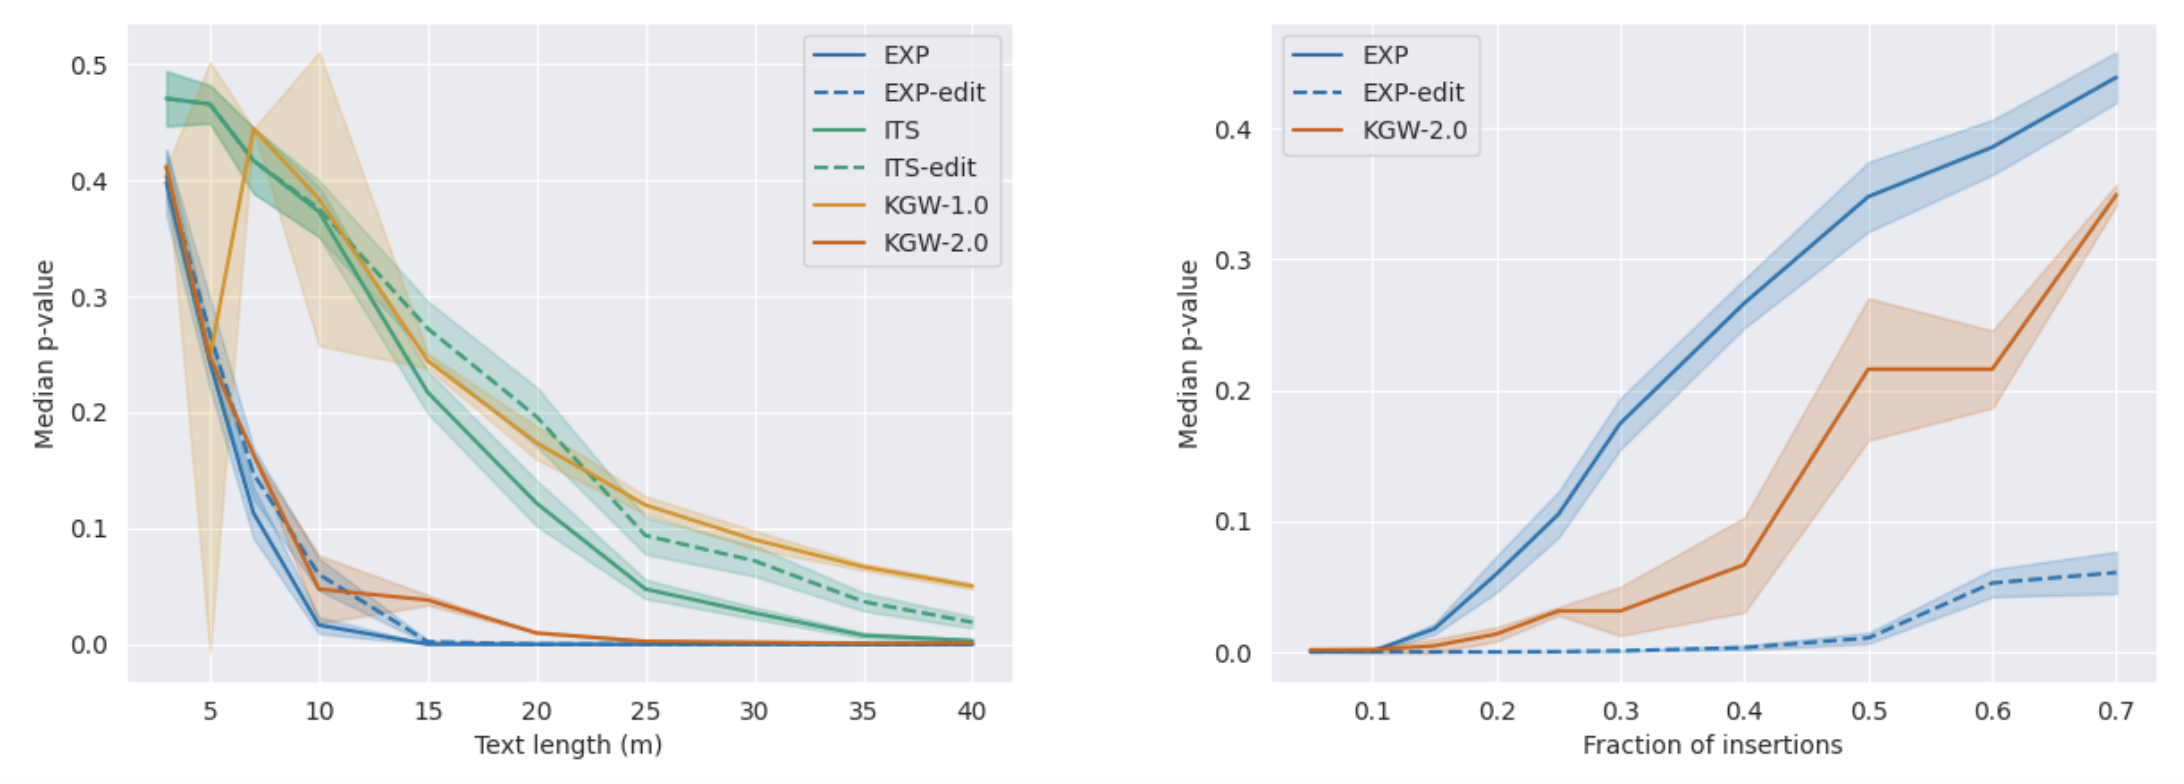
\includegraphics[width=0.8\linewidth]{./images/experiment-method-comparison.png}
        \caption{\footnotesize Comparing Exp-min \& ITS (with and without Levenshtein) and Kirchenbauer et al. \cite{kuditipudi2023robustarticle}.}
        \label{fig:method-comparison}
    \end{figure}
\end{frame}

%-------------------------------------------------
\begin{frame}{Generation Process}
    \begin{enumerate}
        \item \textbf{Key generation.}\;
              A $n$-token private key \(\xi\) is drawn once and stored
              (\(\xi_i\!\sim\!\text{U}(0,1)^{|\mathcal V|}\)).
        \item \textbf{Random shift.}\;
              Before each generation, sample an offset
              \(\tau\sim\text{U}\{0,n-1\}\) and set
              \[
                  \texttt{shift}(\xi,\tau)
                  \;=\;
                  (\xi_\tau,\xi_{\tau+1},\dots,\xi_{\tau+m-1}),
              \]
              implemented with a Mersenne-Twister seeded by the same private
              key.  The shift keeps the watermark distortion-free but
              prevents key-reuse across calls.
        \item \textbf{Token sampling.}\;
              At step \(i\) use Exp-Min with the shifted
              key vector \(\xi_{i}\) to draw
              \(t_i^\star\).  High-probability LM tokens remain likely;
              ties between similarly-probable tokens are biased toward
              lower \(\xi\) values, yielding the hidden correlation.
        \item \textbf{Detection.}\;
              Given text \(\mathbf t\), compute
              cost and compare it to the
              same cost under random surrogate keys; a small p-value
              (\(p<0.01\)) signals a watermark.
    \end{enumerate}
\end{frame}

%-------------------------------------------------
\begin{frame}{Token-selection example}
    \small
    Prompt: \emph{Steganography is the practice of hiding}, \(\tau=41\),
    \begin{center}
        \begin{tabular}{lcccc}
            \textbf{token}      &
            \(\,p_{\text{LM}}\) &
            \(\xi\)             &
            \(p_{\text{WM}}\propto e^{-\frac{\ln\xi}{p_{\text{LM}}}}\) \\ \hline
            messages            & 0.2000 & 0.5555 & 0.1517             \\
            information         & 0.1943 & 0.7710 & \textbf{0.7513}    \\
            data                & 0.1500 & 0.3428 & 0.0023             \\
            a                   & 0.1323 & 0.2594 & 0.0001             \\
            secret              & 0.1252 & 0.1291 & $\ll10^{-4}$       \\
            the                 & 0.0290 & 0.8610 & 0.0165             \\
            ...                 & ...    & ...    & ...                \\
        \end{tabular}
    \end{center}
    The Exp-Min decoder selects \textbf{``information''}. Note that \emph{messages} and \emph{information} had similar
    LM probabilities, but the $\xi$ factor of \emph{information}
    makes it far more likely under the watermark. Unlikely tokens don't suddenly turn likely through the watermark, making it distoriton free.
\end{frame}
